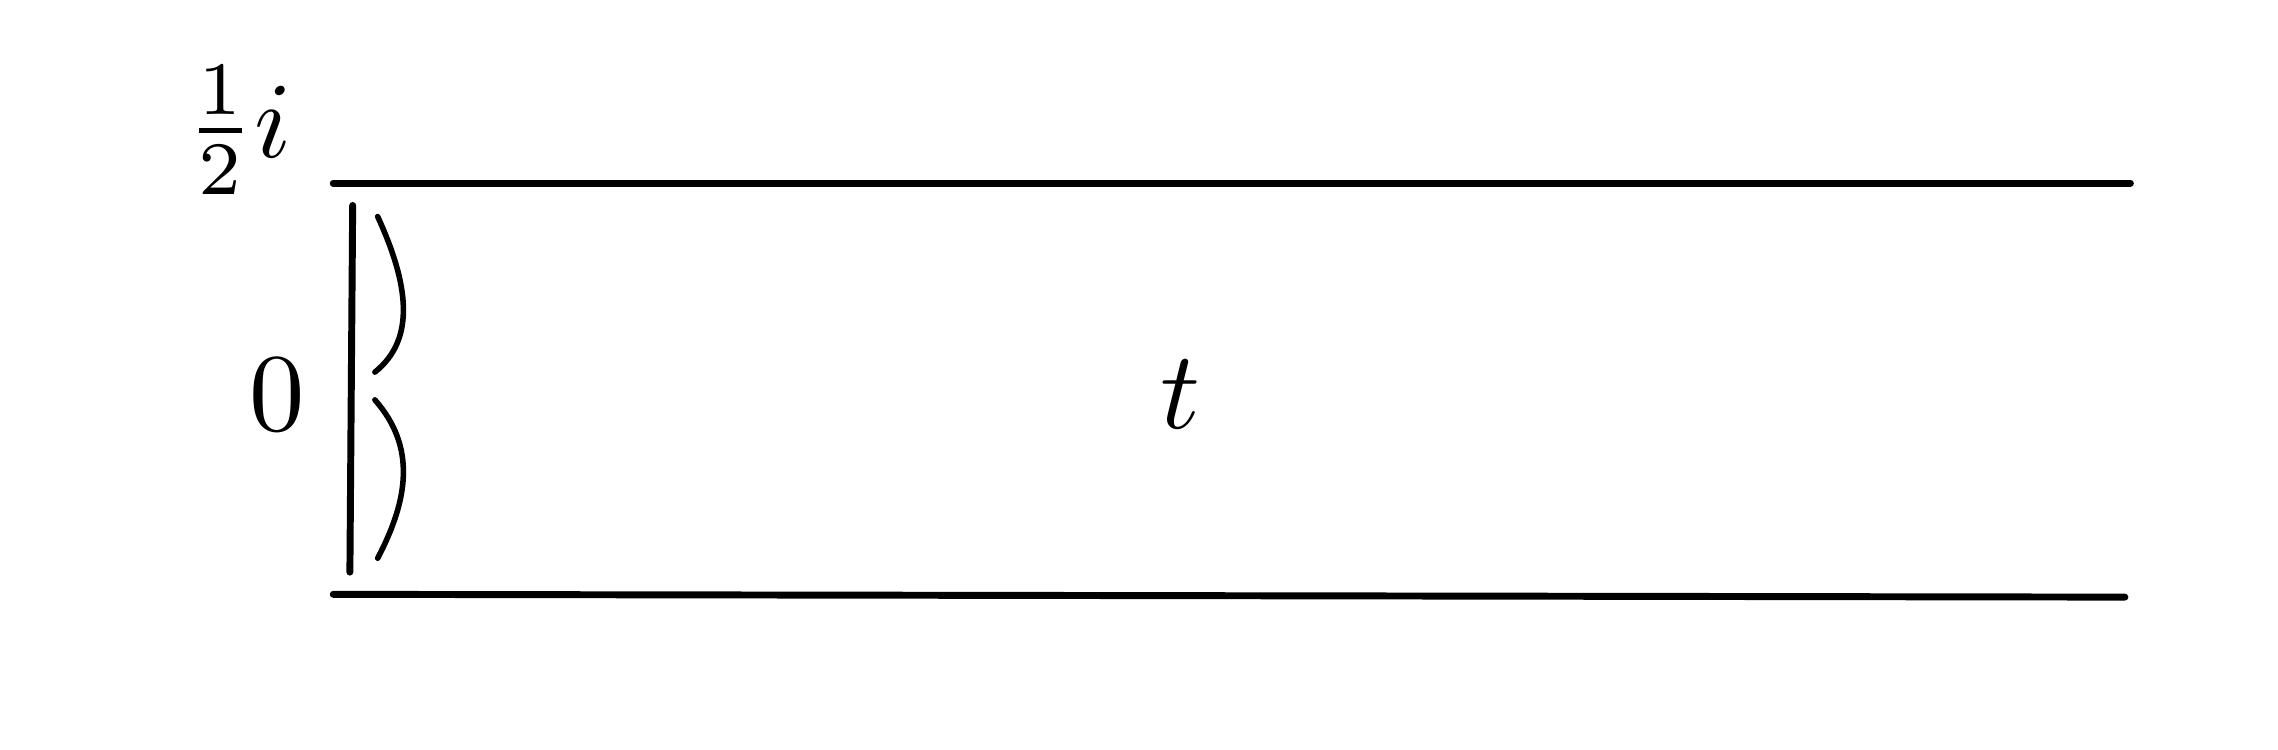
\begin{tikzpicture}[x=1bp,y=-1bp,line cap=round,line join=round]
\path[use as bounding box] (0,0) rectangle (800,250);
\begin{pgfinterruptboundingbox}
\draw[line width=2.5bp] (110,56) -- (757,56);
\draw[line width=2.5bp] (110,204) -- (755,205);
\draw[line width=2.5bp] (117,64) -- (116,196);
\draw[line width=2bp] (126,68) .. controls (137,92) and (140,112.0) .. (125,124.0);
\draw[line width=2bp] (125,134.0) .. controls (140,151.0) and (137,170) .. (126,191);
\node[inner sep=0pt,outer sep=0pt,rotate=0] at (76,37) {\scalebox{3.9}{\ensuremath{\frac12 i}}};
\node[inner sep=0pt,outer sep=0pt,rotate=0] at (90,132) {\scalebox{4}{\ensuremath{0}}};
\node[inner sep=0pt,outer sep=0pt,rotate=0] at (415,132) {\scalebox{4}{\ensuremath{t}}};
\end{pgfinterruptboundingbox}
\end{tikzpicture}
